\chapter{提案手法}\label{chap:method}

\section{概要}
経験則としてなくしものは手に持っていたものを置いて次の動作に移るとき, 置いたこと
%@@@↑語順が悪くて主語がどれかぱっとわかりません。あと人も主語だと思いますが抜けてます。@@@
を忘れることで発生する.
例えば郵便受けから新聞紙をとろうと手に持っていたスマートフォンを床に置いたらその
まま忘れた, といった状況がありうる.
この経験則を次のようにモデル化する.
\begin{itemize}
    \item
    人はマルコフ連鎖に従い行動する.
    \item
    マルコフ連鎖の各状態は寝る, 食べる, 新聞を取るといった動作に対応する.
    \item
    なくしものは異なる動作に遷移するときに確率的に発生する.
\end{itemize}

%@@@↑ひとつひとつちゃんと説明しましょう。@@@

\begin{figure}[H]
    \begin{center}
    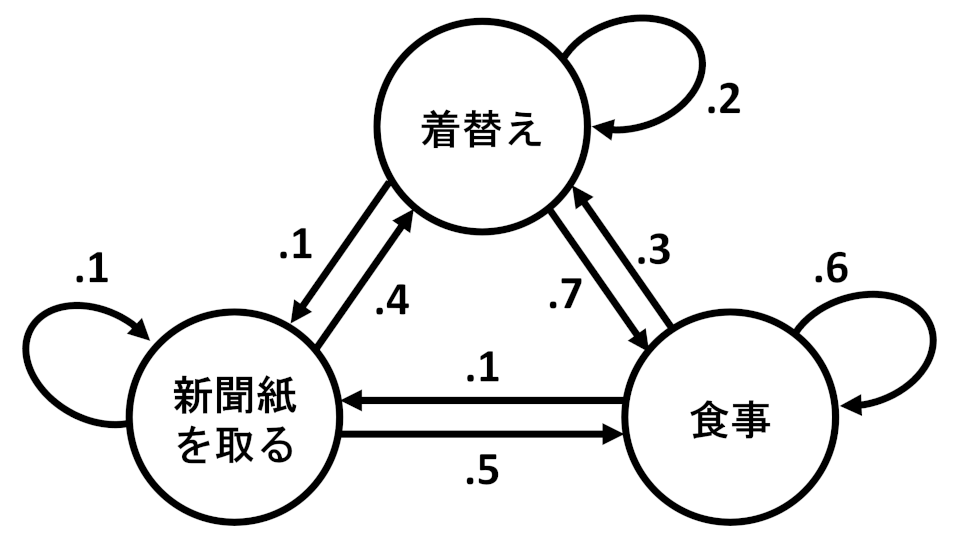
\includegraphics[width=0.6\linewidth]{figs/model_1.png}
    \caption{動作を状態とするマルコフ連鎖のイメージ}
    \label{fig:model1}
    \end{center}
\end{figure}

\begin{figure}[H]
    \begin{center}
    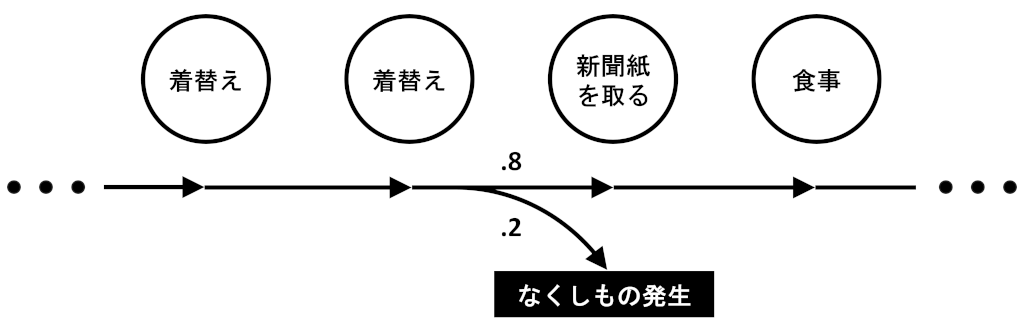
\includegraphics[width=0.8\linewidth]{figs/model_2.png}
    \caption{なくしもの発生のイメージ}
    \label{fig:model2}
    \end{center}
\end{figure}

このモデルの下では遷移を繰り返すことでいつかはなくしものが発生する.
そのため動作ごとになくしものが発生したときに遷移先がその動作である確率を計算でき
る.
この確率をなくしもの発生確率と呼ぶ.

%@@@ここらへんは下書きかな?@@@

動作ごとに利用者がいる位置の傾向を表す分布を用意
なくしもの発生確率を重みとして利用者位置分布を加算
和をなくしものの位置の分布とする

利用者位置分布とマルコフ連鎖を通じてなくしものが発生していない状況下での利用者の行動を反映

\section{定式化}
捜索範囲を$ X \subseteq \mathbb{R}^d \  (d=2,3)$とおく.
%@@@dは2なの3なの?@@@
マルコフ連鎖の状態数すなわち動作の数を$ n $, 各動作を$ m_i\ (i=1,2,\cdots ,n)$, 
$ t \in \{0,1,2,\cdots\} $回目の遷移の後の動作を$ M_t $とおく.ただし$ M_0 $は初期動作とする. 
%@@@↑ここらへん、行をたっぷり使って数式を1行1行書いていいですよ@@@
$ m_i $から$ m_j $に遷移する確率$ \mathrm{P}(M_t = m_j | M_{t-1} = m_i) $を$ a_{i j} $, 
初期動作が$ m_i $である確率$ \mathrm{P}(M_0 = m_i) $を$ s_i $とおく. 
ただしマルコフ連鎖はエルゴード的であると仮定する. \cite{funaki}
%@@@↑引用はピリオドの前(うしろの文の頭にかかっているように見える)@@@
また$ R_t\ (t=1,2,3,\cdots) $を$ 0 $または$ 1 $をとる確率変数とする. 
$ \mathrm{P}(R_t = 0 | M_t = m_j , M_{t - 1} = m_i) $を$ m_i $から$ m_j $への遷移失敗確率と呼ぶ. 
この確率は$ i = j $のとき$ 0 $, $ i \ne j $のとき$ M_j $にのみ依存した$ 0 $より真に大きい値をとると仮定しその値を$ \theta_j $とおく. %@@@行を変える場合も数式は文の中に(「値を<改行>(数式)<改行>とおく。」みたいに)@@@
\begin{equation}
    \mathrm{P}(R_t = 0 | M_t = m_j , M_{t - 1} = m_i) =
    \begin{cases}
        0        & \text{if $i = j$}\\
        \theta_j & \text{if $i \ne j$}
    \end{cases}
\end{equation}
はじめて$ R_t = 0 $となるときになくしものが発生するとし, そのような$ t $を$ \tau $とおく. 
すなわち$ \tau $は任意の$ t^{\prime} \in \{1,2,3,\cdots,t-1\} $に対し$ R_{t^{\prime}} = 0 $かつ$ R_t = 1 $を満たす$ t $である. 
$ \mathrm{P}(\tau < \infty , M_{\tau} = m_i) $を$ p_i $とおき$ m_i $におけるなくしもの発生確率と呼ぶ. 
各記号の補足として図 (\ref{fig:a}) , (\ref{fig:r}) , (\ref{fig:p}) を載せる. 
%↑図の番号に()をつけると数式と区別がつかなくなります。@@@

\begin{figure}[H]
    \begin{center}
    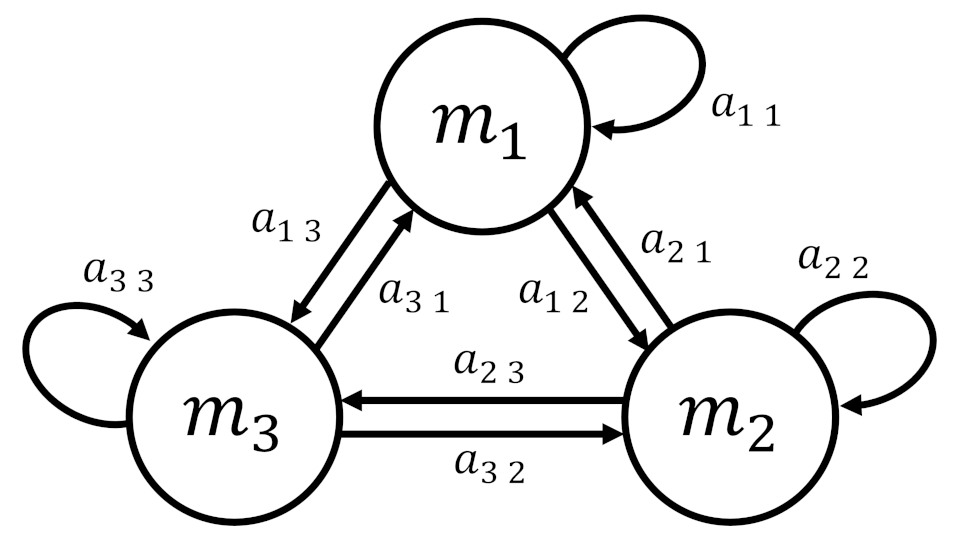
\includegraphics[width=0.5\linewidth]{figs/tr_prob.png}
    \caption{遷移確率$a_{i j}$}
    \label{fig:a}
    \end{center}
\end{figure}

\begin{figure}[H]
    \begin{center}
    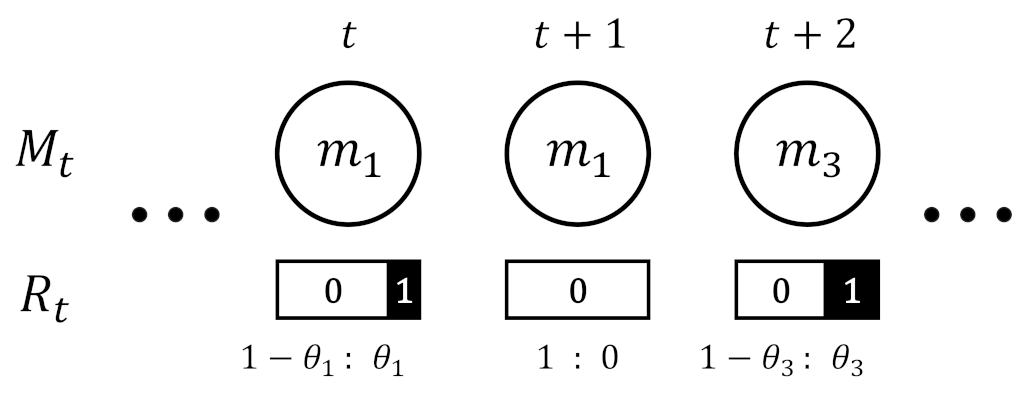
\includegraphics[width=0.8\linewidth]{figs/miss_prob.png}
    \caption{遷移失敗確率, $R_t$が$1$となる確率は前の動作が同じ場合$0$, 異なる場合$\theta_i$}
    \label{fig:r}
    \end{center}
\end{figure}

\begin{figure}[H]
    \begin{center}
    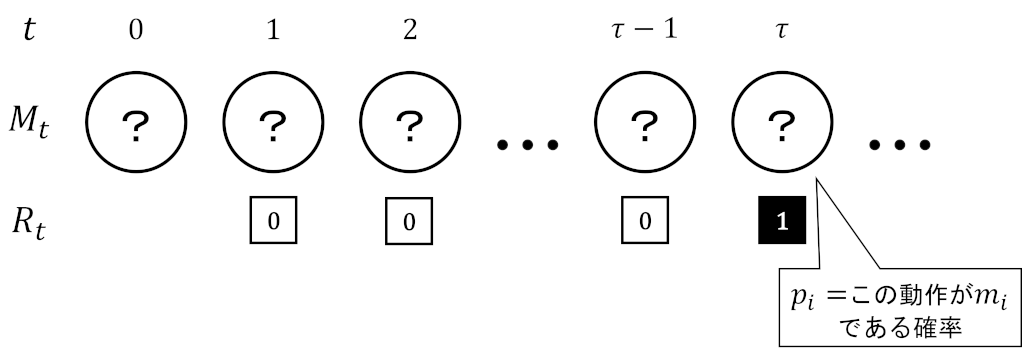
\includegraphics[width=1.0\linewidth]{figs/lost_prob.png}
    \caption{なくしもの発生確率$p_i$}
    \label{fig:p}
    \end{center}
\end{figure}

なくしもの発生確率$ p_i $は下式で求まる. 
\begin{equation} \label{eq:p}
\V{p} = \V{L}(\V{I}-\V{K})^{-1}\V{s}
\end{equation}
ただし
\begin{align*}
\V{p} &= (p_1,p_2,\cdots,p_n)^\mathrm{T} \\
\V{L} &=
\begin{pmatrix}
    0 & \theta_1 a_{2 1} & \cdots & \theta_1 a_{n 1} \\
    \theta_2 a_{1 2} & 0 & \cdots & \theta_2 a_{n 2} \\
    \vdots & \vdots & \ddots & \vdots \\
    \theta_n a_{1 n} & \theta_n a_{2 n} & \cdots & 0 \\
\end{pmatrix}
\\
\V{I} &= n行n列の単位行列 \\
\V{K} &=
\begin{pmatrix}
    a_{1 1} & (1 - \theta_1) a_{2 1} & \cdots & (1 - \theta_1) a_{n 1} \\
    (1 - \theta_2) a_{1 2} & a_{2 2} & \cdots & (1 - \theta_2) a_{n 2} \\
    \vdots & \vdots & \ddots & \vdots \\
    (1 - \theta_n) a_{1 n} & (1 - \theta_n) a_{2 n} & \cdots & a_{n n} \\
\end{pmatrix}
\\
\V{s} &= (s_1,s_2,\cdots,s_n)^\mathrm{T}
\end{align*}
とおいた. 
導出は\ref{sect:proof_p}節にある. 

動作$ m_i $に対応する利用者の位置分布を$ b_i:X \rightarrow [0,\infty) $とし$ \int_X b_i = 1 $を満たすとする. 
利用者位置分布をなくしもの発生確率で重み付けした和$ \sum_i p_i b_i $を$ h $とおき, なくしもの位置分布と呼ぶ. 

\section{学習}
$ s_i, a_{i j}, b_i $について, これらはマルコフ連鎖と位置分布の組み合わせであり連続型HMM(Hidden Markov Model)に類似していることに注目する. 
HMMのパラメータ学習アルゴリズムにBaum-Welchアルゴリズムがある. \cite{ishii_ueda}
$ b_i $が多変量ガウス分布であるという制約の下, 利用者の位置を監視しBaum-Welchアルゴリズムを適用することで$ s_i, a_{i j}, b_i $を同時に学習する. 

$ \theta_i $の学習にはベイズ推論を用いる.
なくしものの発見場所を$ \V{x}_{\mathrm{found}} $, $ \V{\theta} = (\theta_1 , \theta_2 , \cdots , \theta_n)^\mathrm{T} $の事前分布の密度関数を$ f $とおく.
$ \V{\theta} $の分布の更新にあたり尤度としてなくしもの位置分布$ h $を用いる. 
すなわち事後分布の密度関数$ f(\V{\theta} | x_{\mathrm{found}}) $を下式で定める. 
\begin{equation} \label{eq:new_f}
    f(\V{\theta} | \V{x}_{\mathrm{found}}) \propto h(\V{x}_{\mathrm{found}} , \V{\theta}) f(\V{\theta})
\end{equation}
ただし$ h $を$ \V{x} \in X $と$ \V{\theta} $の関数とみなしている. 

\section{推定}
\begin{equation} \label{eq:exp}
    E_{\V{\theta}} [h] = \int_{0}^{1} \int_{0}^{1} \cdots \int_{0}^{1} h f(\theta) \mathrm{d}\theta_1 \mathrm{d}\theta_2 \cdots \mathrm{d}\theta_n
\end{equation}
を推定結果とする. 
